\chapter{Numerical Methods for the Parabolic Two-Temperature Model}
\label{ch:numerical-methods}

\section{Parameter scaling and dimensionless formulation}
\label{sec:ch2-scaling}

Equation \eqref{eq:ch1-pttm} is the studied pTTM under the sub-ablation regime, where $H_m \rightarrow 0$.
In its dimensional form, the model couples temperature-dependent transport coefficients, electron--phonon exchange, and the volumetric heat source of \eqref{eq:ch1-ulp_heat_source}. For the gold closures summarised in \S\ref{sec:ch1-absorption} and \eqref{eq:ch1-heat_conductivity_approx}--\eqref{eq:ch1-ceg-piecewise}, the relevant scales range from picoseconds in time to micrometres in space, while the electron temperature may rise by several orders of magnitude above ambient. A dimensionless reformulation is therefore introduced so that the discrete operators developed later act on variables of comparable magnitude and the diffusion, coupling, and source contributions can be separated cleanly.

Let $T_{\mathrm{ref}}$ denote a representative temperature rise, $t_{\mathrm{ref}}$ a characteristic pulse or observation time, $L_{\mathrm{ref}}$ a characteristic length, and $F_{\mathrm{ref}}$ a reference fluence. For the gold test cases collected in Table~\ref{tab:ch2-params}, the natural choices are the pulse-duration scale for $t_{\mathrm{ref}}$ and the film-thickness scale for $L_{\mathrm{ref}}$, while $T_{\mathrm{ref}}$ is chosen so that both thermal fields remain of order unity over the computational window. We define the dimensionless variables by
\begin{equation}
    u = \frac{T_e}{T_{\mathrm{ref}}}, \qquad
    v = \frac{T_l}{T_{\mathrm{ref}}}, \qquad
    t^* = \frac{t}{t_{\mathrm{ref}}}, \qquad
    x^* = \frac{x}{L_{\mathrm{ref}}}, \qquad
    z^* = \frac{z}{L_{\mathrm{ref}}}, \qquad
    F^* = \frac{F}{F_{\mathrm{ref}}}.
\end{equation}
After the scaling is introduced, the stars are dropped for brevity.

Applying the above change of variables to the reduced forms of \eqref{eq:ch1-pttm} obtained after the dimensionality reductions following \eqref{eq:ch1-ulp_heat_source}, we arrive at the dimensionless parabolic two-temperature model posed on the space--time cylinder
\[
    Q_{\tau_f} \coloneqq \Omega \times (0,\tau_f],
    \qquad
    \Omega \coloneqq [0,1]^d,
    \qquad
    d\in\{1,2,3\},
\]
where \(\tau_f>0\) denotes the dimensionless final time and, under the present scaling choice, \(L_{\mathrm{ref}}=L_x=L_z\).
The governing system reads
\begin{subequations}\label{eq:ch2-dimensionless-pttm}
    \begin{align}
        \partial_t u
         & =
        D_1(u)\,\nabla\!\cdot\!\bigl(K(u,v)\nabla u\bigr)
        - c_1(u)(u-v)
        + s(t,\mathbf{x};u,v),
         &   &
        (t,\mathbf{x})\in Q_{\tau_f},
        \label{eq:ch2-dimensionless-pttm-e}
        \\
        \partial_t v
         & =
        D_2 \nabla^2 v
        + c_2(u)(u-v),
         &   &
        (t,\mathbf{x})\in Q_{\tau_f}.
        \label{eq:ch2-dimensionless-pttm-l}
    \end{align}
\end{subequations}

\paragraph{Geometry convention.}
The dimensional pTTM in \eqref{eq:ch1-pttm} is introduced in the axisymmetric physical geometry, and the source construction in \eqref{eq:ch1-ulp_heat_source} records the corresponding physical energy-deposition model. In Chapter~2, after the scaling and dimensionality reductions described above, the numerical analysis is carried out for the rectangular computational problem \eqref{eq:ch2-dimensionless-pttm} on \(\Omega=[0,1]^d\). Thus the finite-difference operators below are the one-dimensional and Cartesian rectangular operators defined in this chapter.

For the particular case of spatially uniform initial data corresponding to room temperature,
\[
    T_e(\mathbf{x},0)=T_l(\mathbf{x},0)=T_{\mathrm{RT}}=300\,\mathrm{K},
    \qquad \mathbf{x}\in\Omega,
\]
the associated dimensionless initial conditions are
\begin{align}
    u(\mathbf{x},0) & = u_{\mathrm{RT}},
                    &
    v(\mathbf{x},0) & = v_{\mathrm{RT}},
                    &                    & \mathbf{x}\in\Omega,
\end{align}
where
\[
    u_{\mathrm{RT}} = v_{\mathrm{RT}} = \frac{T_{\mathrm{RT}}}{T_{\mathrm{ref}}}.
\]

Moreover, if inhomogeneous Dirichlet boundary conditions are prescribed and held fixed at the same reference state, then
\begin{align}
    u(\mathbf{x},t) & = u_{\mathrm{RT}},
                    &
    v(\mathbf{x},t) & = v_{\mathrm{RT}},
                    &                    & (\mathbf{x},t)\in \partial\Omega \times (0,\tau_f].
\end{align}

\noindent
The constitutive coefficients are inherited from the Chapter~1 closures through
\begin{align}
    D_1(u) & \coloneqq \frac{t_{\mathrm{ref}} k_{e,0}}{L_{\mathrm{ref}}^2 C_e(T_{\mathrm{ref}}u)},  &
    K(u,v) & \coloneqq \frac{k_e(T_{\mathrm{ref}}u, T_{\mathrm{ref}}v)}{k_{e,0}}, \notag              \\
    D_2    & \coloneqq \frac{t_{\mathrm{ref}} k_l}{L_{\mathrm{ref}}^2 C_l},                         &
    c_1(u) & \coloneqq \frac{t_{\mathrm{ref}} G(T_{\mathrm{ref}}u)}{C_e(T_{\mathrm{ref}}u)}, \qquad
    c_2(u) \coloneqq \frac{t_{\mathrm{ref}} G(T_{\mathrm{ref}}u)}{C_l}, \label{eq:ch2-dimensionless-coeffs}
\end{align}
and the dimensionless source is
\begin{equation}
    s(t,\mathbf{x};u,v) \coloneqq \frac{t_{\mathrm{ref}}}{T_{\mathrm{ref}} C_e(T_{\mathrm{ref}}u)}
    S(t_{\mathrm{ref}} t, L_{\mathrm{ref}}\mathbf{x}; T_{\mathrm{ref}}u, T_{\mathrm{ref}}v).
\end{equation}
In the simplified nonlinear model, $D_1$ and $c_1$ are carried by the electron field, $D_2$ is constant, and the temperature dependence of the electron conductivity is isolated in the factor $K(u,v)$.

For the constant-coefficient gold baseline, we adopt the representative values
(see table~\ref{tab:ch2-gold_parameters} for the adopted physical quantities for gold).\footnote{Table 1 in Chen et al. \cite{Chen_2010} provides the physical parameters for Au, Ag, Cu, and Ni}
\begin{equation}
    \label{eq:ch2-linear-params}
    D_1 = 0.0156, \qquad
    D_2 = 1.277 \times 10^{-6}, \qquad
    c_1 = 1.0294, \qquad
    c_2 = 8.4 \times 10^{-3}, \qquad
    K = 1.
\end{equation}
These values define the linear reference problem used for the monolithic Crank--Nicolson benchmarks.

\begin{table}[H]
    \centering
    \begin{tabular}{|l|l|}
        \hline
        \rowcolor{gray!20}
        \textbf{Parameter}                               & \textbf{Value}                                                     \\
        \hline
        Sommerfeld coefficient ($\gamma$)                & 68 J m\textsuperscript{-3} K\textsuperscript{-2}                   \\
        \hline
        Lattice heat capacity ($C_l$)                    & $2.5 \times 10^6$ J m\textsuperscript{-3} K\textsuperscript{-1}    \\
        \hline
        Electron-phonon coupling ($G$)                   & $2.1 \times 10^{16}$ W m\textsuperscript{-3} K\textsuperscript{-1} \\
        \hline
        Electron thermal conductivity at 300K ($k_{e0}$) & 318 W m\textsuperscript{-1} K\textsuperscript{-1}                  \\
        \hline
        Lattice thermal conductivity ($k_l$)             & 3.18 W m\textsuperscript{-1} K\textsuperscript{-1}                 \\
        \hline
        Reference Temperature ($T_R$)                    & 300 K                                                              \\
        \hline
        Electron heat capacity at $T_R$ ($C_e$)          & $2.04 \times 10^4$ J m\textsuperscript{-3} K\textsuperscript{-1}   \\
        \hline
        Material Constant $A_e$                          & $1.18 \times 10^7$ s\textsuperscript{-1} K\textsuperscript{-2}     \\
        \hline
        Material Constant $B_l$                          & $1.25 \times 10^{11}$ s\textsuperscript{-1} K\textsuperscript{-1}  \\
        \hline
    \end{tabular}
    \caption{Physical parameters for gold considered in the simulations.\cite{Chen_2010}}
    \label{tab:ch2-gold_parameters}
\end{table}

For the nonlinear gold model with temperatures below the Sommerfeld's limit, $T (\ll T_m) \ll T_F$, the constitutive factors are approximated by
\begin{align}
    D_1(u) & \simeq \frac{4.6765}{u},          &
    D_2    & = 1.277 \times 10^{-6}, \notag      \\
    c_1(u) & \simeq \frac{0.3088}{u},          &
    c_2(u) & \simeq 8.4 \times 10^{-3}, \qquad
    K(u,v) = \frac{140u}{140v + 5.9u^2}. \label{eq:ch2-variable-params}
\end{align}
The volumetric source is separated into a temperature-independent intensity term and a temperature-dependent attenuation factor,
\begin{equation}
    \label{eq:ch2-source-decomp}
    S_{3D}(t,\varrho,z;u,v) = \mathcal{I}_{3D}(t,\varrho,z;F^*) \, K_{\mathrm{src}}(t,\varrho,z;u,v),
\end{equation}
with
\begin{align}
    \mathcal{I}_{3D}(t,\varrho,z;F^*) & \coloneqq F^* E_{\mathrm{tot}}(t) e^{-\varrho^2/R_0^2} \mathds{1}\{z \ge z_s\}, \notag            \\
    K_{\mathrm{src}}(t,\varrho,z;u,v) & \coloneqq \alpha'(u,v)\bigl(1-R(u,v)\bigr)e^{-\alpha'(u,v)(z-z_s)} b\bigl(L_z;\alpha'(u,v)\bigr).
\end{align}
Here $\alpha'$ and $b$ are the ballistic-corrected absorption coefficient and finite-thickness factor already defined in \eqref{eq:ch1-alpha-prime} and \eqref{eq:ch1-thickness-factor},
while the optical response $R$ follows the constitutive discussion of \S\ref{sec:ch1-absorption}.\footnote{For simplicity, one can let $\alpha \simeq 77.993$ and $R \simeq 0.974$ as suggested in Chen et al. \cite{Chen_2010}.}
In the one-dimensional reduction, where $\varrho \mapsto 0$ and $z \mapsto x$, the dimensionless source used by the solver in the gold benchmark is
\begin{equation}
    \begin{aligned}
        s(t,x;u,v) = {} & 4.6078 \times 10^{-5} e^{-0.0277(t-30)^2}
        \bigl(1-R(u,v)\bigr)\alpha'(u,v)                                        \\
                        & \times \frac{e^{-x\alpha'(u,v)}}{1-e^{-\alpha'(u,v)}}
        \begin{cases}
            1,     & \text{constant coefficients}, \\
            0.3/u, & \text{variable coefficients}.
        \end{cases}
    \end{aligned}
\end{equation}

\begin{table}[htbp]
    \centering
    \caption{Simulation parameters for the gold benchmark problems used throughout Chapter~2.}
    \label{tab:ch2-params}
    \small
    \begin{tabular}{@{}lcccc@{}}
        \toprule
        \rowcolor{gray!20}
        \textbf{Parameter}           & \textbf{1D linear}      & \textbf{2D linear} & \textbf{1D nonlinear} & \textbf{2D nonlinear} \\
        \midrule
        Film width ($\mu$m)          & --                      & 1                  & --                    & 1                     \\
        Film thickness ($\mu$m)      & \multicolumn{4}{c}{1}                                                                        \\
        Evolution time (ps)          & \multicolumn{4}{c}{100}                                                                      \\
        Spatial grid points ($N_x$)  & 201                     & 101                & 201                   & 101                   \\
        Depth grid points ($N_z$)    & --                      & 101                & --                    & 101                   \\
        Temporal grid points ($N_t$) & 1001                    & 201                & 1001                  & 201                   \\
        Laser fluence (J\,m$^{-2}$)  & \multicolumn{4}{c}{100}                                                                      \\
        Pulse duration (ps)          & \multicolumn{4}{c}{10}                                                                       \\
        Beam radius factor ($R_0$)   & --                      & 4                  & --                    & 4                     \\
        \bottomrule
    \end{tabular}
\end{table}

\section{Semi-discrete formulation}
\label{sec:ch2-semidiscrete}

After the scaling of \S\ref{sec:ch2-scaling}, the spatial discretisation of the pTTM is cast in the abstract multiphysics form used by Huang et al.\ \cite{Huang_2019}. Let $\mathbf{u}^i(t) \in \mathbb{R}^{N_i}$ denote the semi-discrete state vector of subsystem $i$, and let $\mathbf{c}^i$ collect the coupling data received from the remaining subsystems. The generic two-field semi-discrete problem is then
\begin{subequations}\label{eq:ch2-abstract-ode}
    \begin{align}
        \dot{\mathbf{u}}^i & = \mathbf{r}^i\bigl(\mathbf{u}^i, \mathbf{c}^i, t\bigr), \qquad t \in (0, \tau_f], \label{eq:ch2-abstract-ode-a} \\
        \mathbf{c}^i       & = \mathbf{c}^i\bigl(\{\mathbf{u}^l\}_{l \in [m]}, t\bigr), \qquad i \in [m]. \label{eq:ch2-abstract-ode-b}
    \end{align}
\end{subequations}
Equation \eqref{eq:ch2-abstract-ode} is the common starting point for the linear monolithic Crank--Nicolson scheme and the nonlinear IMEX partitioned scheme. In particular, the velocity term $\mathbf{r}$ is the semi-discrete counterpart of the differential operators in \eqref{eq:ch2-dimensionless-pttm},
\begin{equation*}
    \partial_t u^i = \mathcal{L}^i(u^i, c^i, x, t), \quad Q_{\tau_f}^i \coloneqq \Omega^i(c^i) \times (0,\tau_f], \quad \forall i \in [m],
\end{equation*}
whereas the predictor $\tilde{\mathbf{c}}$ introduced below determines which parts of the coupling are lagged and which are kept current at each stage.

Following Huang et al., the right-hand side or velocity term is split additively into an explicit correction and an implicit part,
\begin{equation}
    \mathbf{r}\bigl(\mathbf{u}, \mathbf{c}(\mathbf{u},t), t\bigr)
    = \mathbf{f}(\mathbf{u}, \tilde{\mathbf{c}}, t) + \mathbf{g}(\mathbf{u}, \tilde{\mathbf{c}}, t),
\end{equation}
with the formal definitions
\begin{subequations}\label{eq:ch2-imex-split}
    \begin{align}
        \mathbf{f}(\mathbf{u}, \tilde{\mathbf{c}}, t) & \coloneqq \mathbf{r}\bigl(\mathbf{u}, \mathbf{c}(\mathbf{u},t), t\bigr) - \mathbf{r}(\mathbf{u}, \tilde{\mathbf{c}}, t), \label{eq:ch2-imex-split-f} \\
        \mathbf{g}(\mathbf{u}, \tilde{\mathbf{c}}, t) & \coloneqq \mathbf{r}(\mathbf{u}, \tilde{\mathbf{c}}, t). \label{eq:ch2-imex-split-g}
    \end{align}
\end{subequations}
The decomposition is deliberately predictor-based: $\mathbf{g}$ contains the full semi-discrete system evaluated with the predicted coupling data, while $\mathbf{f}$ is the correction required to recover the true coupling. This is the additive IMEX structure that later permits a partitioned solve without discarding the monolithic formulation.

\noindent
In general, the predictor depends on the instantaneous state vector $\mathbf{u}(t)$ and data $\bar{\mathbf{u}}$, stemming from the history of the state vector $\{\mathbf{u}(\tau) \mid \tau < t \}$
\begin{equation}
    \tilde{\mathbf{c}} = \tilde{\mathbf{c}}(\mathbf{u}, \bar{\mathbf{u}}, t) \ .
\end{equation}

For an $s$-stage IMEX Runge--Kutta scheme with timestep $\Delta_t \equiv \Delta_{t^n} \coloneqq t_n - t_{n-1}, \ \forall n\in[N_t]$ for $N_t$ segments and stage times $t_{n,j}$, the update reads \cite{Huang_2019}
\begin{subequations}\label{eq:ch2-imex-rk}
    \begin{align}
        \mathbf{u}_n           & = \mathbf{u}_{n-1} + \sum_{p=1}^{s} \hat{b}_p \hat{\mathbf{k}}_{n,p} + \sum_{p=1}^{s} b_p \mathbf{k}_{n,p}, \label{eq:ch2-imex-rk-a}                     \\
        \hat{\mathbf{k}}_{n,j} & = \Delta_t \, \mathbf{f}\bigl(\mathbf{u}_{n,j}, \tilde{\mathbf{c}}(\mathbf{u}_{n,j}, \mathbf{u}_{n-1}, t_{n,j}), t_{n,j}\bigr), \label{eq:ch2-imex-rk-b} \\
        \mathbf{k}_{n,j}       & = \Delta_t \, \mathbf{g}\bigl(\mathbf{u}_{n,j}, \tilde{\mathbf{c}}(\mathbf{u}_{n,j}, \mathbf{u}_{n-1}, t_{n,j}), t_{n,j}\bigr), \label{eq:ch2-imex-rk-c} \\
        \mathbf{u}_{n,j}       & = \mathbf{u}_{n-1}
        + \sum_{p=1}^{j-1} \hat{a}_{jp} \hat{\mathbf{k}}_{n,p}
        + \sum_{p=1}^{j} a_{jp} \mathbf{k}_{n,p}. \label{eq:ch2-imex-rk-d}
    \end{align}
\end{subequations}
The vectors $\hat{\mathbf{k}}_{n,j}$ and $\mathbf{k}_{n,j}$ are the explicit and implicit stage increments, respectively.

\noindent
The coefficients $\hat{b}_p$, $b_p$, $\hat{a}_{jp}$, and $a_{jp}$ are obtained from the Butcher tableau for the s-stage implicit-explicit Runge-Kutta scheme (IMEX-RK) supplied below.

\begin{table}[H]
    \centering
    \begin{tabular}{c|ccccc}
        \multicolumn{5}{c}{Explicit Runge-Kutta coefficients}                                     \\[0.5ex]
        $0$         &                &                &          &                                \\
        $\hat{c}_2$ & $\hat{a}_{21}$ &                &          &                                \\
        $\hat{c}_3$ & $\hat{a}_{31}$ & $\hat{a}_{32}$ &          &                                \\
        $\vdots$    & $\vdots$       &                & $\ddots$ &                                \\
        $\hat{c}_s$ & $\hat{a}_{s1}$ & $\hat{a}_{s2}$ & $\cdots$ & $\hat{a}_{ss-1}$               \\
        \cline{1-6}
                    & $\hat{b}_1$    & $\hat{b}_2$    & $\cdots$ & $\hat{b}_{s-1}$  & $\hat{b}_s$
    \end{tabular}
    \hspace{5em}
    \begin{tabular}{c|ccccc}
        \multicolumn{6}{c}{Implicit Runge-Kutta coefficients}             \\[0.5ex]
        $c_1$    &          &          &          &            &          \\
        $c_2$    & $a_{21}$ & $a_{22}$ &          &            &          \\
        $c_3$    & $a_{31}$ & $a_{32}$ & $a_{33}$ &            &          \\
        $\vdots$ & $\vdots$ &          & $\ddots$ &            &          \\
        $c_s$    & $a_{s1}$ & $a_{s2}$ & $\cdots$ & $a_{ss-1}$ & $a_{ss}$ \\
        \cline{1-6}
                 & $b_1$    & $b_2$    & $\cdots$ & $b_{s-1}$  & $b_s$
    \end{tabular}
    \caption{Butcher Tableau for s-stage implicit-explicit Runge-Kutta scheme.\cite{Ascher_1997}}
    \label{tab:butcher}
\end{table}

The coupling predictor determines whether the resulting partitioned algorithm is Jacobi- or Gauss--Seidel-type and whether the coupling is weak or strong \cite{Huang_2019}. Weak predictors exclude the diagonal sensitivity $\partial \tilde{\mathbf{c}}^i / \partial \mathbf{u}^i$, whereas strong predictors retain it. Jacobi predictors are block diagonal in the subsystem ordering and admit parallel subsystem solves, while Gauss--Seidel predictors are block triangular and therefore enforce sequential subsystem solves. For the two-field case, the strong Gauss--Seidel predictor produces the lower-triangular Jacobian
%
\begin{equation*}
    \frac{\partial \tilde{\mathbf{c}}}{\partial \mathbf{u}} =
    \begin{bmatrix}
        \frac{\partial \mathbf{c}^1}{\partial \mathbf{u}^1} &        &                                                     \\
        \vdots                                              & \ddots &                                                     \\
        \frac{\partial \mathbf{c}^m}{\partial \mathbf{u}^1} & \cdots & \frac{\partial \mathbf{c}^m}{\partial \mathbf{u}^m}
    \end{bmatrix},
\end{equation*}
%
which implies that the Jacobian of the monolithic implicit system is also block lower triangular
%
\begin{equation*}
    D_{\mathbf{u}^j} \mathbf{g}^i =
    \left\{
    \begin{array}{ll}
        \frac{\partial \mathbf{r}^i}{\partial \mathbf{u}^i} + \frac{\partial \mathbf{r}^i}{\partial \mathbf{c}^i}\frac{\partial \mathbf{c}^i}{\partial \mathbf{u}^i} & i=j \\
        \frac{\partial \mathbf{r}^i}{\partial \mathbf{c}^i}\frac{\partial \mathbf{c}^i}{\partial \mathbf{u}^j}                                                       & i>j \\
        \mathbf{0}                                                                                                                                                   & i<j \\
    \end{array}
    \right.
\end{equation*}
%
This property is the algebraic reason that the monolithic IMEX discretisation can be solved sequentially.
In Kennedy's additive Runge--Kutta nomenclature \cite{Kennedy_2003},
the nonlinear scheme adopted later is a two-stage ARK method with this strong Gauss--Seidel predictor.

For the pTTM, we identify subsystem $1$ with the electron field and subsystem $2$ with the lattice field, that is,
\begin{equation}
    \mathbf{u}^1 = \mathbf{u}, \qquad \mathbf{u}^2 = \mathbf{v}.
\end{equation}
At the semi-discrete level, the two residual operators are written as
\begin{align}
    \mathbf{r}^1(\mathbf{u}, \mathbf{v}, t) & = \mathbf{d}_e(\mathbf{u}, \mathbf{v}) - \mathbf{C}_1(\mathbf{u})(\mathbf{u}-\mathbf{v}) + \mathbf{s}(t,\mathbf{u},\mathbf{v}), \label{eq:ch2-r1} \\
    \mathbf{r}^2(\mathbf{u}, \mathbf{v}, t) & = \mathbf{d}_l(\mathbf{v}) + \mathbf{C}_2(\mathbf{u})(\mathbf{u}-\mathbf{v}), \label{eq:ch2-r2}
\end{align}
where $\mathbf{d}_e$ and $\mathbf{d}_l$ denote the discrete diffusion operators and
\begin{equation}
    \mathbf{C}_1(\mathbf{u}) \coloneqq \operatorname{diag}\bigl(c_1(u_i)\bigr), \qquad
    \mathbf{C}_2(\mathbf{u}) \coloneqq \operatorname{diag}\bigl(c_2(u_i)\bigr).
\end{equation}
The strong Gauss--Seidel predictor specialises to
\begin{equation}
    \tilde{\mathbf{c}}^1(\mathbf{u}_{n,j}, \mathbf{u}_n, t_{n,j}) = \mathbf{c}(\mathbf{u}_{n,j}^1, \mathbf{v}^n), \qquad
    \tilde{\mathbf{c}}^2(\mathbf{u}_{n,j}, \mathbf{u}_n, t_{n,j}) = \mathbf{c}(\mathbf{u}_{n,j}^1, \mathbf{u}_{n,j}^2).
\end{equation}
Consequently,
the electron solve at time level $n+1$ uses the lagged lattice state $\mathbf{v}^n$, whereas the lattice solve uses the just-updated electron state $\mathbf{u}^{n+1}$.
This is the partitioned sequencing embodied in Algorithm~5 of Huang et al.\ \cite{Huang_2019}, restated below for clarity,
and it is the abstraction that underpins the Crank--Nicolson and IMEX schemes developed in the remainder of the chapter.

\begin{algorithm}[H]
    \caption{IMEX-RK partitioned multiphysics scheme: strong Gauss-Seidel predictor \cite{Huang_2019}}
    \label{alg:ch2-strong_GS}
    \begin{algorithmic}[1]
        \For{stages $j \in [s]$}
        \For{physical systems $i \in [m]$}
        \State Define stage solution: $\boldsymbol{u}_{n,j}^i \gets \boldsymbol{u}_{n-1}^i + \sum_{p=1}^{j-1} \hat{a}_{jp} \hat{\boldsymbol{k}}_{n,p}^i + \sum_{p=1}^{j} a_{jp} \boldsymbol{k}_{n,p}^i$
        \State Explicit solve: $\hat{\boldsymbol{k}}_{n,j}^i \gets \Delta_t \boldsymbol{f}^i(\boldsymbol{u}_{n,j}^i, \boldsymbol{c}^i(\boldsymbol{u}_{n,j}^1, \dots, \boldsymbol{u}_{n,j}^i, \boldsymbol{u}_{n-1}^{i+1}, \dots, \boldsymbol{u}_{n-1}^m, t_{n,j}), t_{n,j})$
        \State Implicit solve: $\boldsymbol{k}_{n,j}^i \gets \Delta_t \boldsymbol{g}^i(\boldsymbol{u}_{n,j}^i, \boldsymbol{c}^i(\boldsymbol{u}_{n,j}^1, \dots, \boldsymbol{u}_{n,j}^i, \boldsymbol{u}_{n-1}^{i+1}, \dots, \boldsymbol{u}_{n-1}^m, t_{n,j}), t_{n,j})$
        \EndFor
        \EndFor
        \State Set final solution: $\boldsymbol{u}_n \gets \boldsymbol{u}_{n-1} + \sum_{p=1}^{s} \hat{b}_p \hat{\boldsymbol{k}}_{n,p} + \sum_{p=1}^{s} b_p \boldsymbol{k}_{n,p}$
    \end{algorithmic}
\end{algorithm}

\section{Spatial discretisation}
\label{sec:ch2-spatial}

The fully discrete schemes are built from second-order centred finite differences on uniform one- and two-dimensional grids. In one spatial dimension, with grid points $x_i=i\Delta_x$, the discrete Laplacian is
\begin{equation}
    \mathcal{L}[u]_i \coloneqq \frac{u_{i+1} - 2u_i + u_{i-1}}{\Delta_x^2}.
    \label{eq:ch2-laplacian-1d}
\end{equation}
This is the standard second-difference operator appearing in the linear gold benchmark.

On the rectangular two-dimensional grid $(x_i,z_j)$ with spacings $\Delta_x$ and $\Delta_z$, the Laplacian becomes
\begin{equation}
    \mathcal{L}[u]_{i,j}
    \coloneqq
    \frac{u_{i+1,j} - 2u_{i,j} + u_{i-1,j}}{\Delta_x^2}
    +
    \frac{u_{i,j+1} - 2u_{i,j} + u_{i,j-1}}{\Delta_z^2}.
    \label{eq:ch2-laplacian-2d}
\end{equation}
After vectorisation, the same operator has the Kronecker representation
\[
    \mathbf{L}_{2D}
    =
    \mathbf{I}_{N_z} \otimes \mathbf{L}_x
    +
    \mathbf{L}_z \otimes \mathbf{I}_{N_x},
\]
where $\mathbf{L}_x$ and $\mathbf{L}_z$ are the one-dimensional second-difference matrices in the $x$- and $z$-directions, respectively.

For the nonlinear electron diffusion term, the conductivity is evaluated at cell faces using arithmetic averaging, following Kadioglu et al.\ \cite{Kadioglu_2008}. In one dimension,
\begin{equation}
    \mathcal{K}(K)[u]_i
    \coloneqq
    \frac{1}{\Delta_x}
    \left[
    K_{i+\frac{1}{2}} \frac{u_{i+1}-u_i}{\Delta_x}
    -
    K_{i-\frac{1}{2}} \frac{u_i-u_{i-1}}{\Delta_x}
    \right],
    \qquad
    K_{i\pm\frac{1}{2}} \coloneqq \frac{K_i + K_{i\pm1}}{2}.
    \label{eq:ch2-flux-divergence}
\end{equation}
When $K$ is constant, one recovers $\mathcal{K}(K)[u]_i = K \mathcal{L}[u]_i$, so the nonlinear operator reduces to the standard Laplacian up to the constant conductivity factor.

Dirichlet boundary conditions are imposed directly in the algebraic systems by identity-row replacement. If $\mathbf{M}$ denotes the discrete system matrix and $\mathbf{b}$ the right-hand side, then for each boundary row $r \in \partial \Omega_h$,
\begin{equation}
    \mathbf{M}_{r,:} = \mathbf{e}_r^\top,
    \qquad
    \mathbf{b}_r = g_r^{n+1},
\end{equation}
where $g_r^{n+1}$ is the prescribed boundary value at the new timestep. The same construction is used for the one-dimensional end points and for all boundary edges in the two-dimensional problem.

\section{Linear schemes: monolithic Crank--Nicolson}
\label{sec:ch2-linear}

\subsection{One-dimensional linear scheme}
\label{sec:ch2-linear-1d}

Starting from the semi-discrete system \eqref{eq:ch2-abstract-ode} with constant coefficients \eqref{eq:ch2-linear-params}, the one-dimensional linear pTTM reads
\begin{equation}
    \dot{u}_i = F_1[u,v]_i, \qquad \dot{v}_i = F_2[u,v]_i,
\end{equation}
with
\begin{align}
    F_1[u,v]_i & \coloneqq D_1 \mathcal{L}[u]_i - c_1(u_i-v_i) + s_i(u,v), \notag \\
    F_2[u,v]_i & \coloneqq D_2 \mathcal{L}[v]_i + c_2(u_i-v_i).
\end{align}
Applying Crank--Nicolson to both subsystems gives
\begin{align}
    \frac{u_i^{n+1} - u_i^n}{\Delta_t}
     & =
    \frac{1}{2}\bigl(F_1[u^{n+1},v^{n+1}]_i + F_1[u^n,v^n]_i\bigr), \notag \\
    \frac{v_i^{n+1} - v_i^n}{\Delta_t}
     & =
    \frac{1}{2}\bigl(F_2[u^{n+1},v^{n+1}]_i + F_2[u^n,v^n]_i\bigr),
\end{align}
which can be rearranged into the implicit coupled form
\begin{align}
    \left(I - \frac{1}{2} D_1 \Delta_t \mathcal{L}\right)u^{n+1}
    + \frac{1}{2} c_1 \Delta_t (u^{n+1} - v^{n+1})
     & =
    u^n
    + \frac{1}{2} D_1 \Delta_t \mathcal{L}[u^n]
    - \frac{1}{2} c_1 \Delta_t (u^n - v^n) \notag                              \\
     & \quad
    + \frac{1}{2} \Delta_t \bigl[s(u^{n+1},v^{n+1}) + s(u^n,v^n)\bigr], \notag \\
    - \frac{1}{2} c_2 \Delta_t (u^{n+1} - v^{n+1})
    + \left(I - \frac{1}{2} D_2 \Delta_t \mathcal{L}\right)v^{n+1}
     & =
    v^n
    + \frac{1}{2} D_2 \Delta_t \mathcal{L}[v^n]
    + \frac{1}{2} c_2 \Delta_t (u^n - v^n). \notag
\end{align}

Collecting the spatial unknowns into $\mathbf{u}^{n+1}, \mathbf{v}^{n+1} \in \mathbb{R}^{N_x}$ yields the monolithic block system
\begin{equation}
    \begin{bmatrix}
        \mathbf{A}_e + c_e \mathbf{I} & -c_e \mathbf{I}               \\
        -c_l \mathbf{I}               & \mathbf{A}_l + c_l \mathbf{I}
    \end{bmatrix}
    \begin{bmatrix}
        \mathbf{u}^{n+1} \\
        \mathbf{v}^{n+1}
    \end{bmatrix}
    =
    \begin{bmatrix}
        \mathbf{b}_e \\
        \mathbf{b}_l
    \end{bmatrix},
    \label{eq:ch2-block-1d}
\end{equation}
where
\begin{align}
    \mathbf{A}_e
     & \coloneqq \mathbf{I} - \frac{1}{2} D_1 \Delta_t \mathbf{L}_{1D}, \qquad
    \mathbf{A}_l \coloneqq \mathbf{I} - \frac{1}{2} D_2 \Delta_t \mathbf{L}_{1D}, \notag \\
    c_e
     & \coloneqq \frac{1}{2} c_1 \Delta_t, \qquad
    c_l \coloneqq \frac{1}{2} c_2 \Delta_t, \notag                                       \\
    \mathbf{b}_e
     & \coloneqq
    \mathbf{u}^n
    + \frac{1}{2} D_1 \Delta_t \mathbf{L}_{1D}\mathbf{u}^n
    - c_e(\mathbf{u}^n - \mathbf{v}^n)
    + \frac{1}{2} \Delta_t
    \bigl(
    \mathbf{s}(\mathbf{u}^{n+1}, \mathbf{v}^{n+1})
    +
    \mathbf{s}(\mathbf{u}^n, \mathbf{v}^n)
    \bigr), \notag                                                                       \\
    \mathbf{b}_l
     & \coloneqq
    \mathbf{v}^n
    + \frac{1}{2} D_2 \Delta_t \mathbf{L}_{1D}\mathbf{v}^n
    + c_l(\mathbf{u}^n - \mathbf{v}^n). \notag
\end{align}
Although the transport and coupling coefficients are constant, the electron right-hand side still depends on $\mathbf{u}^{n+1}$ and $\mathbf{v}^{n+1}$ through the source evaluation, $\mathbf{s}(\mathbf{u}^{n+1}, \mathbf{v}^{n+1})$.
The resulting system is therefore solved by Picard iteration rather than by a single linear solve.

\subsection{Two-dimensional linear scheme}
\label{sec:ch2-linear-2d}

The two-dimensional constant-coefficient model follows the same construction with the Laplacian \eqref{eq:ch2-laplacian-2d}. Writing the semi-discrete system componentwise gives
\begin{align}
    \dot{u}_{i,j} & = D_1 \mathcal{L}[u]_{i,j} - c_1(u_{i,j} - v_{i,j}) + s_{i,j}(u,v), \notag \\
    \dot{v}_{i,j} & = D_2 \mathcal{L}[v]_{i,j} + c_2(u_{i,j} - v_{i,j}),
\end{align}
and Crank--Nicolson again yields a coupled implicit update of the same form as in the one-dimensional case. After vectorising the fields into $\mathbf{u}^{n+1}, \mathbf{v}^{n+1} \in \mathbb{R}^{M}$ with $M \coloneqq N_x N_z$, one obtains
\begin{equation}
    \begin{bmatrix}
        \mathbf{A}_e^{(2D)} + c_e \mathbf{I} & -c_e \mathbf{I}                      \\
        -c_l \mathbf{I}                      & \mathbf{A}_l^{(2D)} + c_l \mathbf{I}
    \end{bmatrix}
    \begin{bmatrix}
        \mathbf{u}^{n+1} \\
        \mathbf{v}^{n+1}
    \end{bmatrix}
    =
    \begin{bmatrix}
        \mathbf{b}_e \\
        \mathbf{b}_l
    \end{bmatrix},
    \label{eq:ch2-block-2d}
\end{equation}
with
\begin{equation*}
    \mathbf{A}_e^{(2D)} \coloneqq \mathbf{I} - \frac{1}{2} D_1 \Delta_t \mathbf{L}_{2D}, \quad
    \mathbf{A}_l^{(2D)} \coloneqq \mathbf{I} - \frac{1}{2} D_2 \Delta_t \mathbf{L}_{2D}.
\end{equation*}
The right-hand-side vectors $\mathbf{b}_e$ and $\mathbf{b}_l$ have the same structure as in \eqref{eq:ch2-block-1d}, with $\mathbf{L}_{1D}$ replaced by the Kronecker-assembled operator $\mathbf{L}_{2D}$. This Kronecker structure is exploited directly in the sparse linear solve, so the passage from one to two spatial dimensions changes the matrix size but not the algebraic form of the monolithic update.

\subsection{Picard iterations with Anderson acceleration}
\label{sec:ch2-picard}

Let
\[
    \mathbf{x}^{(k)}
    \coloneqq
    \begin{bmatrix}
        (\mathbf{u}^{(k)})^\top &
        (\mathbf{v}^{(k)})^\top
    \end{bmatrix}^\top,
\]
and define the fixed-point map associated with the monolithic Crank--Nicolson solve by
\begin{equation}
    \mathbf{x}^{(k+1)} = \mathcal{F}\bigl[\mathbf{x}^{(k)}\bigr].
\end{equation}
The Picard loop updates the source with the current iterate, solves the resulting linear system, and then accelerates the fixed-point residual by Anderson mixing \cite{Pollock_2018}. The complete procedure is summarised in Algorithm~\ref{alg:ch2-picard}.

\begin{algorithm}[htbp]
    \caption{Monolithic Picard with Anderson acceleration}
    \label{alg:ch2-picard}
    \begin{algorithmic}[1]
        \Require $\mathbf{u}^n$, $\mathbf{v}^n$, monolithic matrix $\mathbf{M}$, Picard tolerance $\tau_{\mathrm{Picard}}$, safety constant $\epsilon_{\mathrm{tol}}$, mixing depth $m$
        \State $\mathbf{x}^{(0)} \gets [(\mathbf{u}^n)^\top, (\mathbf{v}^n)^\top]^\top$
        \State $\mathcal{X} \gets \emptyset$, $\mathcal{F} \gets \emptyset$
        \For{$k=0,1,2,\ldots,k_{\max}-1$}
        \State Evaluate $\mathbf{s}^{(k)} \gets \mathbf{s}(\mathbf{u}^{(k)}, \mathbf{v}^{(k)})$
        \State Assemble $\mathbf{b}_e^{(k)}$, $\mathbf{b}_l^{(k)}$, and $\mathbf{b}^{(k)}$
        \State Solve $\mathbf{M}\mathbf{x}^{(k+1)}_{\mathrm{raw}} = \mathbf{b}^{(k)}$
        \State $\mathbf{f}^{(k)} \gets \mathbf{x}^{(k+1)}_{\mathrm{raw}} - \mathbf{x}^{(k)}$
        \If{$k=0$ \textbf{or} $m=0$ \textbf{or} $|\mathcal{F}|<2$}
        \State $\mathbf{x}^{(k+1)} \gets \mathbf{x}^{(k+1)}_{\mathrm{raw}}$
        \Else
        \State $m_k \gets \min(m, |\mathcal{F}|-1)$ and $s \gets |\mathcal{F}|-m_k$
        \State Build $\Delta \mathbf{F}$ and $\Delta \mathbf{X}$ from the most recent $m_k$ history vectors
        \State Solve $(\Delta \mathbf{F}^\top \Delta \mathbf{F} + \epsilon \mathbf{I})\boldsymbol{\gamma} = \Delta \mathbf{F}^\top \mathbf{f}^{(k)}$
        \State $\mathbf{x}^{(k+1)} \gets \mathbf{x}^{(k+1)}_{\mathrm{raw}} - \Delta \mathbf{X}\boldsymbol{\gamma}$
        \State $\mathbf{x}^{(k+1)} \gets (1-\beta)\mathbf{x}^{(k)} + \beta \mathbf{x}^{(k+1)}$
        \EndIf
        \If{$\dfrac{\|\mathbf{x}^{(k+1)}-\mathbf{x}^{(k)}\|_2}{\|\mathbf{x}^{(k)}\|_2+\epsilon_{\mathrm{tol}}} < \tau_{\mathrm{Picard}}$}
        \State \textbf{break}
        \EndIf
        \State Append $\mathbf{x}^{(k)}$ to $\mathcal{X}$ and $\mathbf{f}^{(k)}$ to $\mathcal{F}$, truncating to at most $m+1$ entries (FIFO).
        \EndFor
        \Ensure $\mathbf{x}^{(k+1)} = [(\mathbf{u}^{n+1})^\top, (\mathbf{v}^{n+1})^\top]^\top$
    \end{algorithmic}
\end{algorithm}

The Anderson step is obtained by solving the regularised least-squares problem
\begin{equation}
    \boldsymbol{\gamma}
    =
    \arg\min_{\boldsymbol{\alpha}}
    \left\{
    \|\Delta \mathbf{F}\boldsymbol{\alpha} - \mathbf{f}^{(k)}\|_2^2
    +
    \epsilon \|\boldsymbol{\alpha}\|_2^2
    \right\},
\end{equation}
followed by the correction
\begin{equation}
    \mathbf{x}^{(k+1)} = \mathbf{x}^{(k+1)}_{\mathrm{raw}} - \Delta \mathbf{X}\boldsymbol{\gamma},
    \qquad
    \mathbf{x}^{(k+1)} \leftarrow (1-\beta)\mathbf{x}^{(k)} + \beta \mathbf{x}^{(k+1)}.
\end{equation}
The parameter values used throughout the linear and nonlinear monolithic solves are listed in Table~\ref{tab:ch2-picard-params}.

\begin{table}[htbp]
    \centering
    \caption{Algorithmic fixed-point iteration parameters used in the monolithic solves.}
    \label{tab:ch2-picard-params}
    \begin{tabular}{@{}ll@{}}
        \toprule
        \rowcolor{gray!20}
        \textbf{Parameter}        & \textbf{Value}                       \\
        \midrule
        Maximum Picard iterations & $30$                                 \\
        Convergence tolerance     & $\tau_{\mathrm{Picard}} = 10^{-6}$   \\
        Anderson mixing depth     & $m = 5$                              \\
        Anderson relaxation       & $\beta = 1.0$                        \\
        Safety constant           & $\epsilon_{\mathrm{tol}} = 10^{-16}$ \\
        Regularisation            & $\epsilon = 10^{-8}$                 \\
        \bottomrule
    \end{tabular}
\end{table}

For the two-dimensional system, the same algorithm applies after replacing $N_x$ by $M = N_xN_z$ and using the matrix \eqref{eq:ch2-block-2d}. The only substantive difference is the increased size of the sparse block system; the fixed-point structure and Anderson acceleration remain unchanged.

\section{Nonlinear schemes: IMEX Heun--Crank--Nicolson with strong Gauss--Seidel predictor}
\label{sec:ch2-nonlinear}

\subsection{LCS operator decomposition and IMEX splitting}
\label{sec:ch2-imex-split}

For the nonlinear pTTM it is convenient to collect the two thermal fields into the block vector
\[
    \boldsymbol{\theta}
    \coloneqq
    \begin{bmatrix}
        \mathbf{u} \\
        \mathbf{v}
    \end{bmatrix},
\]
and to decompose the semi-discrete velocity into diffusion, coupling, and source contributions. In the notation of \eqref{eq:ch2-r1}--\eqref{eq:ch2-r2}, this yields the LCS split
\begin{subequations}\label{eq:ch2-lcs-split}
    \begin{align}
        \mathbf{F}(\boldsymbol{\theta},t)
         & =
        \mathbf{L}(\boldsymbol{\theta})[\boldsymbol{\theta}]
        +
        \mathbf{C}(\boldsymbol{\theta})[\boldsymbol{\theta}]
        +
        \mathbf{S}(t,\boldsymbol{\theta}),
        \label{eq:ch2-lcs-split-a} \\
        \mathbf{L}(\boldsymbol{\theta})
         & \coloneqq
        \begin{bmatrix}
            D_1(\mathbf{u})\mathcal{K}(K)[\mathbf{u}] & \mathbf{0}                  \\
            \mathbf{0}                                & D_2 \mathcal{L}[\mathbf{v}]
        \end{bmatrix},
        \label{eq:ch2-lcs-split-b} \\
        \mathbf{C}(\boldsymbol{\theta})
         & \coloneqq
        \begin{bmatrix}
            -\mathbf{C}_1(\mathbf{u}) & \mathbf{C}_1(\mathbf{u})  \\
            \mathbf{C}_2(\mathbf{u})  & -\mathbf{C}_2(\mathbf{u})
        \end{bmatrix},
        \label{eq:ch2-lcs-split-c} \\
        \mathbf{S}(t,\boldsymbol{\theta})
         & \coloneqq
        \begin{bmatrix}
            \mathbf{s}(t,\mathbf{u},\mathbf{v}) \\
            \mathbf{0}
        \end{bmatrix}.
        \label{eq:ch2-lcs-split-d}
    \end{align}
\end{subequations}
The block \(\mathbf{L}\) is diagonal and contains the stiff diffusion operators, \(\mathbf{C}\) contains the off-diagonal electron--phonon exchange, and \(\mathbf{S}\) contains the laser source acting only on the electron subsystem.

The additive IMEX decomposition \eqref{eq:ch2-imex-split} is now specialised so that the implicit part \(\mathbf{g}\) carries the stiff diffusion and coupling terms evaluated with the strong Gauss--Seidel predictor,
whereas the explicit part \(\mathbf{f}\) carries the correction to the predictor together with the non-stiff source contribution.
Equivalently, the adopted split is ``implicit diffusion + coupling, explicit source''.
Since \(\mathbf{S}(t,\boldsymbol{\theta})\) is bounded and non-stiff over the fluence range of interest,
it is advanced by the explicit Heun part without degrading the practical behaviour of the scheme;
the resulting accuracy and runtime are checked empirically in \S\ref{sec:ch2-stability}.

\begin{table}[htbp]
    \centering
    \caption{Butcher tableaux for the two-stage ARK2(1)2[2]SA scheme: explicit trapezoidal (Heun) and implicit trapezoidal (Crank--Nicolson). The implicit part is A-stable and stiffly accurate (SA) by construction. \cite{Ascher_1997,Kennedy_2003}}
    \label{tab:ch2-butcher}
    \begin{minipage}[t]{0.42\textwidth}
        \centering
        \begin{tabular}{@{}c|cc@{}}
            \multicolumn{3}{c}{Explicit (Heun)}               \\[0.5ex]
            $0$               & $0$           & $0$           \\
            $1$               & $1$           & $0$           \\
            \cline{1-3}
            \rule{0pt}{2.5ex} & $\frac{1}{2}$ & $\frac{1}{2}$
        \end{tabular}
    \end{minipage}
    \hfill
    \begin{minipage}[t]{0.42\textwidth}
        \centering
        \begin{tabular}{@{}c|cc@{}}
            \multicolumn{3}{c}{Implicit (CN)}                 \\[0.5ex]
            $0$               & $0$           & $0$           \\
            $1$               & $\frac{1}{2}$ & $\frac{1}{2}$ \\
            \cline{1-3}
            \rule{0pt}{2.5ex} & $\frac{1}{2}$ & $\frac{1}{2}$
        \end{tabular}
    \end{minipage}
\end{table}

In the terminology of \cite{Kennedy_2003}, this pair is the ARK2(1)2[2]SA scheme: global order \(p=2\), embedded order \(q=1\), \(s=2\) stages, two-part additive split, and stiffly accurate implicit tableau. The implicit trapezoidal part is A-stable but not L-stable, because the Crank--Nicolson stability function does not vanish as the stiff eigenvalue tends to infinity. For the diffusion-dominated parameter regime studied here, however, A-stability is sufficient. The full stage algebra that derives the sequential CN-GS formulae from Algorithm~5 of \cite{Huang_2019} is presented in Appendix~\ref{app:imex-derivation}.

\subsection{Strong Gauss--Seidel predictor: sequential solve}
\label{sec:ch2-strong-gs}

The strong Gauss--Seidel predictor introduced in \S\ref{sec:ch2-semidiscrete} specialises to the two-field pTTM as
\begin{subequations}\label{eq:ch2-gs-predictors}
    \begin{align}
        \tilde{\mathbf{c}}^{1}\big|_{j=1}
         & =
        \mathbf{c}(\mathbf{u}^{n},\mathbf{v}^{n}),
         &
        \tilde{\mathbf{c}}^{2}\big|_{j=1}
         & =
        \mathbf{c}(\mathbf{u}^{n},\mathbf{v}^{n}),
        \label{eq:ch2-gs-predictors-a} \\
        \tilde{\mathbf{c}}^{1}\big|_{j=2}
         & =
        \mathbf{c}(\mathbf{u}^{n}_{*},\mathbf{v}^{n}),
         &
        \tilde{\mathbf{c}}^{2}\big|_{j=2}
         & =
        \mathbf{c}(\mathbf{u}^{n}_{*},\mathbf{v}^{n}_{*}).
        \label{eq:ch2-gs-predictors-b}
    \end{align}
\end{subequations}
At the first stage both predictors coincide with the exact old-time coupling, whereas at the second stage the electron problem retains the lagged lattice field \(\mathbf{v}^{n}\) and the lattice problem uses the updated electron stage value \(\mathbf{u}^{n}_{*}\).

\paragraph{Remark.}
As detailed in Appendix~\ref{app:imex-derivation}, the explicit predictor correction vanishes identically at stage \(j=1\), because \(\mathbf{u}_{n,1}=\mathbf{u}^{n}\), \(\mathbf{v}_{n,1}=\mathbf{v}^{n}\), and hence \(\tilde{\mathbf{c}}^{i}(\boldsymbol{\theta}^{n},\boldsymbol{\theta}^{n})=\mathbf{c}(\boldsymbol{\theta}^{n})\). At stage \(j=2\), the lattice subsystem still has no explicit contribution, while the electron subsystem retains only the explicit source correction associated with the Heun update. Consequently, the stiff part is solved sequentially in Crank--Nicolson form.

\noindent
The recovered stage equations therefore reduce to the sequential CN-GS update
\begin{subequations}\label{eq:ch2-cn-gs-update}
    \begin{align}
        \mathbf{u}^{n+1}
         & =
        \mathbf{u}^{n}
        +
        \frac{\Delta_t}{2}
        \Bigl[
            \mathbf{r}^{1}(\mathbf{u}^{n},\mathbf{v}^{n},t^{n})
            +
            \mathbf{r}^{1}(\mathbf{u}^{n+1},\mathbf{v}^{n},t^{n+1})
            \Bigr],
        \label{eq:ch2-cn-gs-update-a} \\
        \mathbf{v}^{n+1}
         & =
        \mathbf{v}^{n}
        +
        \frac{\Delta_t}{2}
        \Bigl[
            \mathbf{r}^{2}(\mathbf{u}^{n},\mathbf{v}^{n},t^{n})
            +
            \mathbf{r}^{2}(\mathbf{u}^{n+1},\mathbf{v}^{n+1},t^{n+1})
            \Bigr].
        \label{eq:ch2-cn-gs-update-b}
    \end{align}
\end{subequations}
Equation \eqref{eq:ch2-cn-gs-update-a} depicts the electron subsystem being solved with the lattice field lagged to \(\mathbf{v}^{n}\), while \eqref{eq:ch2-cn-gs-update-b} shows that the lattice subsystem uses the updated electron state \(\mathbf{u}^{n+1}\). This is the strong Gauss--Seidel sequential ordering predicted by the lower-triangular Jacobian.

\subsection{One-dimensional nonlinear scheme}
\label{sec:ch2-nonlinear-1d}

In one spatial dimension, the nonlinear semi-discrete equations are
\begin{align}
    \dot{u}_i
     & =
    s(t,x_i;u_i,v_i)
    +
    D_1(u_i)\mathcal{K}(K)[u]_i
    -
    c_1(u_i)(u_i-v_i),
    \notag \\
    \dot{v}_i
     & =
    D_2 \mathcal{L}[v]_i
    +
    c_2(u_i)(u_i-v_i),
    \notag
\end{align}
so that the source is identified as the explicit part,
\[
    \mathbf{F}_1(t,\mathbf{u},\mathbf{v}) \coloneqq \mathbf{s}(t,\mathbf{u},\mathbf{v}),
    \qquad
    \mathbf{F}_2(t,\mathbf{u},\mathbf{v}) \coloneqq \mathbf{0},
\]
whereas the stiff diffusion--coupling operators are
\[
    \mathbf{G}_1(\mathbf{u},\mathbf{v}) \coloneqq D_1(\mathbf{u})\mathcal{K}(K)[\mathbf{u}] - \mathbf{C}_1(\mathbf{u})(\mathbf{u}-\mathbf{v}),
    \qquad
    \mathbf{G}_2(\mathbf{u},\mathbf{v}) \coloneqq D_2 \mathcal{L}[\mathbf{v}] + \mathbf{C}_2(\mathbf{u})(\mathbf{u}-\mathbf{v}).
\]

With the strong Gauss--Seidel predictor and the two-stage Heun/CN pair, the stage equations become
\begin{subequations}\label{eq:ch2-nonlinear-1d-stage}
    \begin{align}
        \mathbf{u}^{n}_{*}
         & =
        \mathbf{u}^{n}
        +
        \frac{\Delta_t}{2}
        \Bigl[
            \mathbf{s}(t^{n},\mathbf{u}^{n},\mathbf{v}^{n})
            +
            \mathbf{s}(t^{n+1},\mathbf{u}^{n}_{*},\mathbf{v}^{n})
            \Bigr]
        +
        \frac{\Delta_t}{2}
        \Bigl[
            \mathbf{G}_1(\mathbf{u}^{n},\mathbf{v}^{n})
            +
            \mathbf{G}_1(\mathbf{u}^{n}_{*},\mathbf{v}^{n}_{*})
            \Bigr],
        \label{eq:ch2-nonlinear-1d-stage-a} \\
        \mathbf{v}^{n}_{*}
         & =
        \mathbf{v}^{n}
        +
        \frac{\Delta_t}{2}
        \Bigl[
            \mathbf{G}_2(\mathbf{u}^{n},\mathbf{v}^{n})
            +
            \mathbf{G}_2(\mathbf{u}^{n}_{*},\mathbf{v}^{n}_{*})
            \Bigr].
        \label{eq:ch2-nonlinear-1d-stage-b}
    \end{align}
\end{subequations}

At Picard iterate \(k\), all nonlinear coefficients are frozen at the current stage guess \((\mathbf{u}^{(k)},\mathbf{v}^{(k)})\). Writing \(K_k \coloneqq K(\mathbf{u}^{(k)},\mathbf{v}^{(k)})\)
and letting \(\mathbf{K}(K_k)\) denote the sparse matrix representation of the flux-divergence operator \(\mathcal{K}(K_k)[\cdot]\), the stage solve is
\begin{equation}
    \begin{bmatrix}
        \mathbf{A}^{e}_{k} + \mathbf{C}^{e}_{k} & -\mathbf{C}^{e}_{k}                     \\
        -\mathbf{C}^{l}_{k}                     & \mathbf{A}^{l}_{k} + \mathbf{C}^{l}_{k}
    \end{bmatrix}
    \begin{bmatrix}
        \mathbf{u}^{(k+1)} \\
        \mathbf{v}^{(k+1)}
    \end{bmatrix}
    =
    \mathbf{b}^{(k)},
    \label{eq:ch2-picard-nonlinear-1d}
\end{equation}
where
\begin{align}
    \mathbf{A}^{e}_{k} & \coloneqq \mathbf{I} - \frac{\Delta_t}{2} D_1(\mathbf{u}^{(k)}) \mathbf{K}(K_k), \qquad
    \mathbf{A}^{l}_{k} \coloneqq \mathbf{I} - \frac{\Delta_t}{2} D_2 \mathbf{L}_{1D}, \notag                     \\
    \mathbf{C}^{e}_{k} & \coloneqq \frac{\Delta_t}{2}\mathbf{C}_1(\mathbf{u}^{(k)}), \qquad
    \mathbf{C}^{l}_{k}
    \coloneqq
    \frac{\Delta_t}{2}\mathbf{C}_2(\mathbf{u}^{(k)}),
    \notag
\end{align}
and
\begin{align}
    \mathbf{b}^{(k)}
     & \coloneqq
    \begin{bmatrix}
        \mathbf{b}^{e,(k)} \\
        \mathbf{b}^{l,(k)}
    \end{bmatrix},
    \notag       \\
    \mathbf{b}^{e,(k)}
     & \coloneqq
    \mathbf{u}^{n}
    +
    \frac{\Delta_t}{2}
    D_1(\mathbf{u}^{n})\mathbf{K}(K(\mathbf{u}^{n},\mathbf{v}^{n}))\mathbf{u}^{n}
    -
    \frac{\Delta_t}{2}
    \mathbf{C}_1(\mathbf{u}^{n})(\mathbf{u}^{n}-\mathbf{v}^{n})
    \notag       \\
     & \quad
    +
    \frac{\Delta_t}{2}
    \Bigl[
        \mathbf{s}(t^{n},\mathbf{u}^{n},\mathbf{v}^{n})
        +
        \mathbf{s}(t^{n+1},\mathbf{u}^{(k)},\mathbf{v}^{n})
        \Bigr],
    \notag       \\
    \mathbf{b}^{l,(k)}
     & \coloneqq
    \mathbf{v}^{n}
    +
    \frac{\Delta_t}{2}
    D_2 \mathbf{L}_{1D}\mathbf{v}^{n}
    +
    \frac{\Delta_t}{2}
    \mathbf{C}_2(\mathbf{u}^{n})(\mathbf{u}^{n}-\mathbf{v}^{n}).
    \notag
\end{align}
The Anderson-accelerated fixed-point iteration of Algorithm~\ref{alg:ch2-picard} applies directly to \eqref{eq:ch2-picard-nonlinear-1d}; only the frozen matrices and right-hand side change from one iterate to the next.

Once the stage problem has converged, the timestep update is
\begin{subequations}\label{eq:ch2-nonlinear-1d-final}
    \begin{align}
        \mathbf{u}^{n+1}
         & =
        \mathbf{u}^{n}
        +
        \frac{\Delta_t}{2}
        \Bigl[
            \mathbf{r}^{1}(\mathbf{u}^{n},\mathbf{v}^{n},t^{n})
            +
            \mathbf{r}^{1}(\mathbf{u}^{n}_{*},\mathbf{v}^{n}_{*},t^{n+1})
            \Bigr],
        \label{eq:ch2-nonlinear-1d-final-a} \\
        \mathbf{v}^{n+1}
         & =
        \mathbf{v}^{n}
        +
        \frac{\Delta_t}{2}
        \Bigl[
            \mathbf{r}^{2}(\mathbf{u}^{n},\mathbf{v}^{n},t^{n})
            +
            \mathbf{r}^{2}(\mathbf{u}^{n}_{*},\mathbf{v}^{n}_{*},t^{n+1})
            \Bigr].
        \label{eq:ch2-nonlinear-1d-final-b}
    \end{align}
\end{subequations}

\subsection{Two-dimensional nonlinear scheme}
\label{sec:ch2-nonlinear-2d}

The two-dimensional nonlinear scheme has the same algebraic structure as the one-dimensional formulation, but with \(M \coloneqq N_xN_z\) unknowns per field and with the discrete operators replaced by their two-dimensional counterparts. In particular, the lattice diffusion uses \(\mathcal{L}[v]_{i,j}\) from \eqref{eq:ch2-laplacian-2d}, while the electron diffusion uses the two-dimensional flux-divergence operator
\[
    \begin{aligned}
        \mathcal{K}(K)[u]_{i,j}
         & =
        \frac{1}{\Delta_x}
        \left[
        K_{i+\frac{1}{2},j}\frac{u_{i+1,j}-u_{i,j}}{\Delta_x}
        -
        K_{i-\frac{1}{2},j}\frac{u_{i,j}-u_{i-1,j}}{\Delta_x}
        \right]  \\
         & \quad
        +
        \frac{1}{\Delta_z}
        \left[
        K_{i,j+\frac{1}{2}}\frac{u_{i,j+1}-u_{i,j}}{\Delta_z}
        -
        K_{i,j-\frac{1}{2}}\frac{u_{i,j}-u_{i,j-1}}{\Delta_z}
        \right].
    \end{aligned}
\]
with arithmetic face averages
\[
    K_{i+\frac{1}{2},j} = \frac{K_{i,j}+K_{i+1,j}}{2},
    \qquad
    K_{i,j+\frac{1}{2}} = \frac{K_{i,j}+K_{i,j+1}}{2},
\]
and analogous definitions on the left and lower faces.

The corresponding Picard solve is the direct extension of \eqref{eq:ch2-picard-nonlinear-1d}:
\begin{equation}
    \begin{bmatrix}
        \mathbf{A}^{e,(2D)}_{k} + \mathbf{C}^{e}_{k} & -\mathbf{C}^{e}_{k}                          \\
        -\mathbf{C}^{l}_{k}                          & \mathbf{A}^{l,(2D)}_{k} + \mathbf{C}^{l}_{k}
    \end{bmatrix}
    \begin{bmatrix}
        \mathbf{u}^{(k+1)} \\
        \mathbf{v}^{(k+1)}
    \end{bmatrix}
    =
    \mathbf{b}^{(k)}_{2D},
    \label{eq:ch2-picard-nonlinear-2d}
\end{equation}
where
\[
    \mathbf{A}^{e,(2D)}_{k}
    \coloneqq
    \mathbf{I}
    -
    \frac{\Delta_t}{2}
    D_1(\mathbf{u}^{(k)}) \mathbf{K}_{2D}(K_k),
    \qquad
    \mathbf{A}^{l,(2D)}_{k}
    \coloneqq
    \mathbf{I}
    -
    \frac{\Delta_t}{2}
    D_2 \mathbf{L}_{2D}.
\]
Thus, only the spatial operator changes from \(\mathbf{L}_{1D}\) to \(\mathbf{L}_{2D}\) and from \(\mathbf{K}(K_k)\) to its two-dimensional counterpart \(\mathbf{K}_{2D}(K_k)\); the IMEX splitting, strong Gauss--Seidel sequencing, Picard iteration, and Anderson acceleration are otherwise unchanged.

\subsection{Damage threshold estimation}
\label{sec:ch2-threshold}

The damage-threshold study estimates the minimum fluence \(F_{\mathrm{th}}\)
for which the peak lattice temperature reaches the melting threshold. Starting
from a prescribed initial value \(F_{\mathrm{init}}\), the algorithm evaluates
trial fluences
\[
    F_j = r^j F_{\mathrm{init}},
    \qquad j = 0,1,2,\dotsc,
\]
until the melting criterion is first satisfied. This exponential-search stage
produces a certified bracket, which is then refined by bisection to the target
fluence tolerance.

The damage threshold results using the exponential--bisection algorithm are
reported in detail in \S\ref{sec:ch3-ablation},
Table~\ref{tab:ch3-threshold-linear}, and
Table~\ref{tab:ch3-threshold-nonlinear}. The theoretical guarantees for this
algorithm are established in Appendix~\ref{app:equilibration-ablation}.

For the retained threshold workflow, this subsection is algorithmic. Each trial fluence is advanced with the schemes described above, the maximum lattice temperature is recorded, and the exponential--bisection loop terminates once the prescribed fluence tolerance is reached. The numerical behaviour of the implementation is checked by the stiffness, refinement, and runtime evidence in \S\ref{sec:ch2-stiffness} and \S\ref{sec:ch2-stability}.

\section{Stiffness analysis}
\label{sec:ch2-stiffness}

For the nonlinear pTTM, the dominant stiffness mechanism is the competition between the variable electron diffusion and the combined electron--phonon/source contribution in \eqref{eq:ch2-r1}.
Under an order-estimation argument, the electron equation may be expanded locally as
\begin{equation}
    \dot{u}
    \approx
    D_1(u)\frac{K(u,v)}{\Delta_x^2}\mathcal{L}[u]
    -
    c_1(u)(u-v)
    +
    \alpha'(u,v)\bigl(1-R(u,v)\bigr)\frac{F^*}{t_p} g(x,t;u,v),
    \label{eq:ch2-stiffness-expansion}
\end{equation}
where \(g(x,t;u,v)\) denotes the bounded spatio-temporal profile inherited from the source decomposition \eqref{eq:ch2-source-decomp}. For resolved solutions, both \(\mathcal{L}[u]\) and \(u-v\) remain \(\mathcal{O}(1)\), so the leading coefficients define the scales
\begin{subequations}\label{eq:ch2-stiffness-terms}
    \begin{align}
        q_1(u,v)
         & \coloneqq
        D_1(u)\frac{K(u,v)}{\Delta_x^2},
        \label{eq:ch2-stiffness-terms-a} \\
        q_2(u,v;F^*)
         & \coloneqq
        -c_1(u)
        +
        \alpha'(u,v)\bigl(1-R(u,v)\bigr)\frac{F^*}{t_p}.
        \label{eq:ch2-stiffness-terms-b}
    \end{align}
\end{subequations}
This yields the stiffness quotient indicator
\begin{equation}
    \lambda(t;F^*)
    \coloneqq
    \max_{x \in \Omega}
    \left\{
    \frac{q_1\bigl(u(t,x),v(t,x)\bigr)}{q_2\bigl(u(t,x),v(t,x);F^*\bigr)}
    \right\},
    \label{eq:ch2-stiffness-ratio}
\end{equation}
for the fluence scaling introduced in \S\ref{sec:ch2-scaling}. Large values \(\lambda \gg 1\) indicate diffusion-dominated stiffness, whereas \(\lambda \ll 1\) indicates that the reaction-plus-source contribution is dominant.

The extrema reported below are
\begin{equation}
    \lambda_{\max}(F^*) \coloneqq \max_t \{\lambda(t;F^*)\},
    \qquad
    \lambda_{\min}(F^*) \coloneqq \min_t \{\lambda(t;F^*)\},
    \label{eq:ch2-stiffness-extrema}
\end{equation}
evaluated for each metal over the simulated time horizon. The physical fluence \(F\) appearing in Table~\ref{tab:ch2-stiffness} is the corresponding laboratory fluence associated with the dimensionless input \(F^*\).

\begin{table}[htbp]
    \centering
    \caption{Stability analysis for the five metals considered in the nonlinear study, with \(t_p = 10\,\mathrm{ps}\) and \(\Delta_x^2 = 2.5 \times 10^{-5}\).}
    \label{tab:ch2-stiffness}
    \small
    \begin{tabular}{@{}lccccc@{}}
        \toprule
        Metal & \(F\) (J/m\(^2\)) & \(\lambda_{\max}\)    & \(t_{\max}\) (ps) & \(\lambda_{\min}\)     & \(t_{\min}\) (ps) \\
        \midrule
        \multirow{6}{*}{Au}
              & 1                 & 670.985               & 0.5               & 670.980                & 32.8              \\
              & 10                & 29.4358               & 0.0               & 29.4353                & 100.0             \\
              & 100               & 2.78713               & 0.0               & 2.78673                & 100.0             \\
              & 1,000             & 0.27724               & 0.0               & 0.27682                & 100.0             \\
              & 10,000            & 0.0277093             & 0.0               & 0.0268501              & 100.0             \\
              & 100,000\(^{*}\)   & 0.00277079            & 0.0               & 0.00234589             & 37.2              \\
        \midrule
        \multirow{6}{*}{Ni}
              & 1                 & 0.0963592             & 27.3              & 0.0963146              & 0.0               \\
              & 10                & 0.0094365             & 27.4              & 0.00938898             & 0.0               \\
              & 100               & 0.000970507           & 26.3              & 0.00093654             & 0.0               \\
              & 1,000             & 0.000117881           & 25.6              & \(9.36\times10^{-5}\)  & 0.0               \\
              & 10,000            & \(1.34\times10^{-5}\) & 21.2              & \(9.36\times10^{-6}\)  & 98.2              \\
              & 100,000\(^{*}\)   & \(1.43\times10^{-6}\) & 18.0              & \(9.36\times10^{-7}\)  & 0.0               \\
        \midrule
        \multirow{7}{*}{Cu}
              & 1                 & 618.839               & 4.1               & 618.838                & 100.0             \\
              & 10                & 20.7478               & 1.8               & 20.7478                & 100.0             \\
              & 100               & 1.94546               & 0.4               & 1.94542                & 100.0             \\
              & 1,000             & 0.193341              & 0.4               & 0.193304               & 100.0             \\
              & 10,000            & 0.0193221             & 0.0               & 0.0192618              & 100.0             \\
              & 100,000           & 0.00193209            & 0.0               & 0.0018518              & 100.0             \\
              & 1,000,000\(^{*}\) & 0.000193208           & 0.0               & \(2.04\times10^{-35}\) & 24.3              \\
        \midrule
        \multirow{7}{*}{Ag}
              & 1                 & 13880                 & 1.6               & 13875.8                & 32.2              \\
              & 10                & 72.1828               & 1.2               & 72.1805                & 100.0             \\
              & 100               & 6.59325               & 0.1               & 6.59139                & 100.0             \\
              & 1,000             & 0.653664              & 0.0               & 0.651802               & 100.0             \\
              & 10,000            & 0.0653104             & 0.0               & 0.0623943              & 100.0             \\
              & 100,000           & 0.00653048            & 0.0               & 0.00316153             & 100.0             \\
              & 1,000,000\(^{*}\) & 0.000653042           & 0.0               & \(5.92\times10^{-11}\) & 24.7              \\
        \midrule
        \multirow{6}{*}{Ti}
              & 1                 & 0.153682              & 0.0               & 0.153682               & 64.7              \\
              & 10                & 0.0126894             & 0.4               & 0.0126894              & 100.0             \\
              & 100               & 0.0012472             & 0.4               & 0.0012472              & 100.0             \\
              & 1,000             & 0.000124507           & 0.4               & 0.000124507            & 100.0             \\
              & 10,000            & \(1.24\times10^{-5}\) & 0.4               & \(1.24\times10^{-5}\)  & 100.0             \\
              & 100,000\(^{*}\)   & \(1.24\times10^{-6}\) & 0.4               & \(1.24\times10^{-6}\)  & 27.5              \\
        \bottomrule
    \end{tabular}

    \vspace{1mm}
    \parbox{0.9\linewidth}{\footnotesize \(^{*}\) Numerical instability produced NaN values in the corresponding simulations, so these datapoints were excluded from the fitted fluence trends.}
\end{table}

\begin{figure}[htbp]
    \centering
    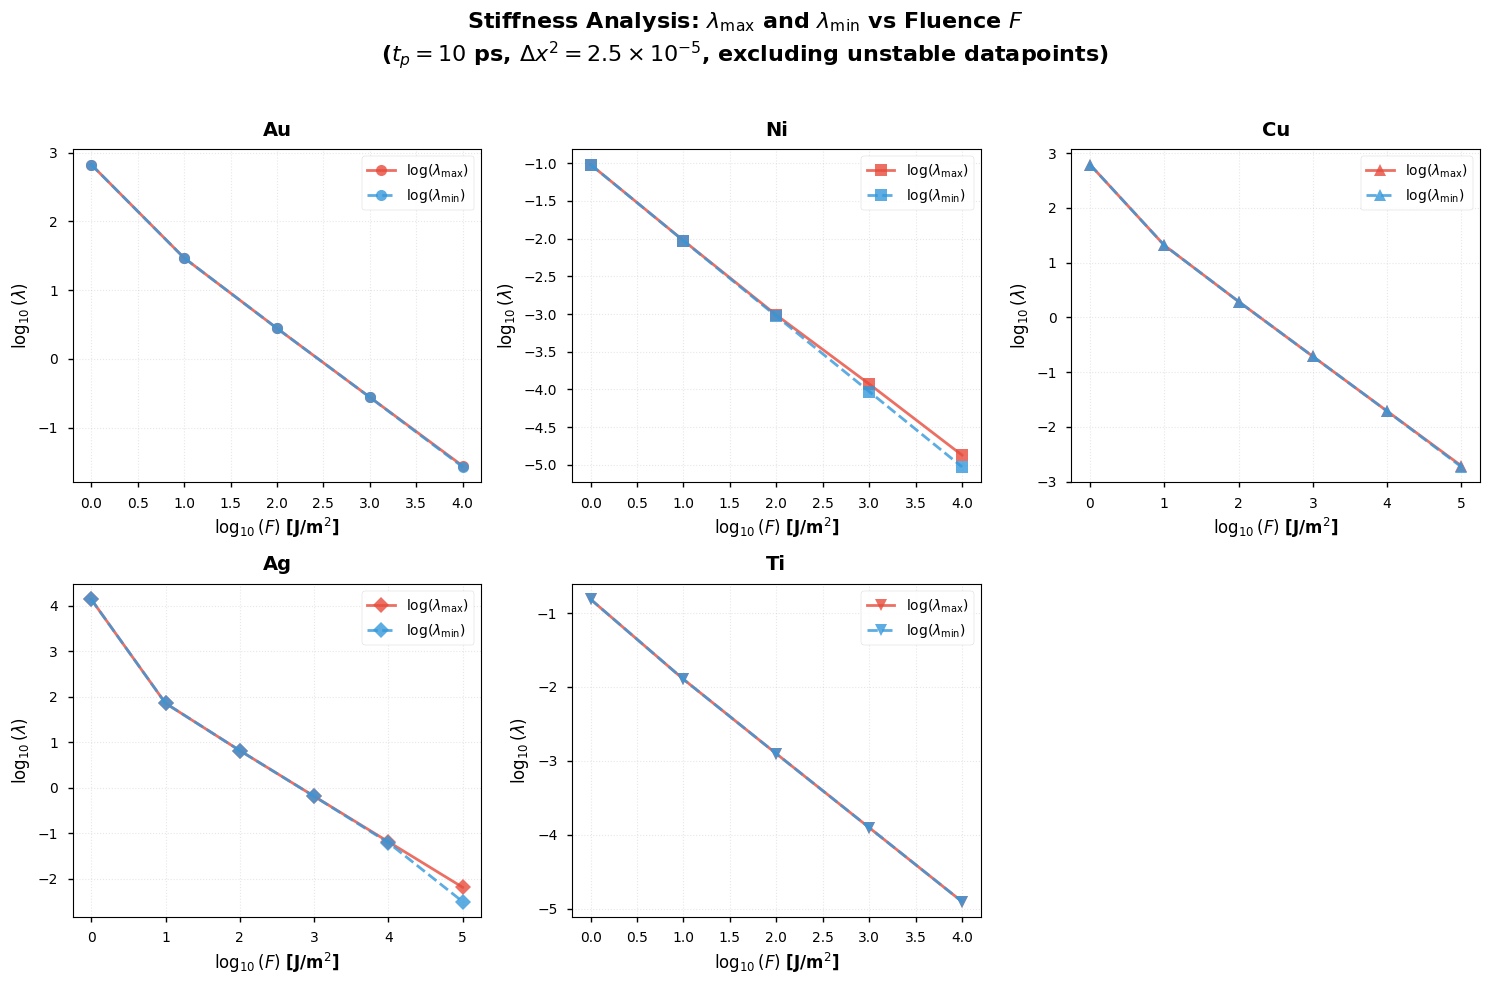
\includegraphics[width=0.95\linewidth]{figures/ch2/stiffness_plots.png}
    \caption{Log-log plots of maximum (\(\lambda_{\max}\)) and minimum (\(\lambda_{\min}\)) stiffness ratios versus physical fluence \(F\) for five metals (Au, Ni, Cu, Ag, Ti). Unstable datapoints are excluded. Power-law slopes from linear regression indicate approximate inverse scaling \(\lambda \propto F^{-1}\) across most metals.}
    \label{fig:ch2-stiffness}
\end{figure}

Figure~\ref{fig:ch2-stiffness} shows that the fitted slopes are close to \(-1\) for all five metals, so increasing fluence weakens the effective diffusion dominance almost inversely. Physically, higher fluence strengthens the reaction-plus-source scale in \eqref{eq:ch2-stiffness-terms-b} more rapidly than the diffusion scale in \eqref{eq:ch2-stiffness-terms-a}, thereby reducing \(\lambda\). Gold and copper exhibit the largest stiffness ratios at low fluence and therefore remain strongly diffusion-dominated in the experimentally relevant regime, whereas nickel and titanium stay in the coupling-dominated range with \(\lambda \ll 1\). This material dependence justifies the IMEX choice made in \S\ref{sec:ch2-nonlinear}: treating diffusion implicitly is essential for Au and Cu, while retaining explicit treatment of the bounded source remains benign across the range studied here.

\section{Numerical results and validation}
\label{sec:ch2-results}

The numerical experiments compare the monolithic Crank--Nicolson discretisations of \S\ref{sec:ch2-linear} with the nonlinear IMEX-CN-GS scheme of \S\ref{sec:ch2-nonlinear}. Table~\ref{tab:ch2-performance} reports the observed runtimes on a local AMD Ryzen~7 5800H CPU (16 logical cores, two threads per core), while Table~\ref{tab:ch2-sim-params} summarises the Au benchmark configuration used to compare the one- and two-dimensional solvers.

\begin{table}[htbp]
    \centering
    \caption{Solver performance comparison for the Au benchmark runs.}
    \label{tab:ch2-performance}
    \begin{tabular}{@{}lccccc@{}}
        \toprule
        Solver       & Steps & Avg. time (s) & Min. (s) & Max. (s) & Total time (s) \\
        \midrule
        1D Linear    & 1000  & 0.0029        & 0.0019   & 0.0054   & 2.9215         \\
        2D Linear    & 200   & 0.0278        & 0.0080   & 0.1030   & 5.6048         \\
        1D Nonlinear & 1000  & 0.0264        & 0.0178   & 0.0397   & 26.3907        \\
        2D Nonlinear & 200   & 1.7819        & 1.2142   & 2.4305   & 54.6500        \\
        \bottomrule
    \end{tabular}

    \vspace{1mm}
    \parbox{0.94\linewidth}{\footnotesize Run on a local CPU (AMD Ryzen~7 5800H with Radeon Graphics, 16 logical cores, two threads per core).}
\end{table}

The runtime increase from the linear solvers to the nonlinear solvers is driven by the coefficient updates and the Anderson-accelerated Picard iterations discussed in \S\ref{sec:ch2-picard}. The most expensive case is the two-dimensional nonlinear solve, which has a reported total runtime of approximately \(55\) s on the stated hardware, but still remains practical for the threshold-study parameter sweeps reported below.

\begin{table}[htbp]
    \centering
    \caption{Simulation parameters for the Au TTM comparison study.}
    \label{tab:ch2-sim-params}
    \begin{tabular}{@{}lcccc@{}}
        \toprule
        Parameter                      & 1D Linear               & 2D Linear & 1D Nonlinear & 2D Nonlinear \\
        \midrule
        Film width (\(\mu\)m)          & --                      & 1         & --           & 1            \\
        Film thickness (\(\mu\)m)      & \multicolumn{4}{c}{1}                                             \\
        Evolution time (ps)            & \multicolumn{4}{c}{100}                                           \\
        Spatial grid points (\(N_x\))  & 201                     & 101       & 201          & 101          \\
        Depth grid points (\(N_z\))    & --                      & 101       & --           & 101          \\
        Temporal grid points (\(N_t\)) & 1001                    & 201       & 1001         & 201          \\
        Laser fluence (J/m\(^2\))      & \multicolumn{4}{c}{100}                                           \\
        Pulse duration (ps)            & \multicolumn{4}{c}{10}                                            \\
        Beam radius factor (\(R_0\))   & --                      & 4         & --           & 4            \\
        \bottomrule
    \end{tabular}
\end{table}

\section{Empirical refinement and performance validation}
\label{sec:ch2-stability}

The schemes developed in \S\S\ref{sec:ch2-linear}--\ref{sec:ch2-nonlinear} are checked here through direct time- and space-refinement studies and through a wall-clock comparison of the candidate IMEX splits. This keeps the validation tied to the computations used later for threshold estimation: the preferred split should retain the expected second-order behaviour while reducing cost relative to a fully implicit solve.

\subsection{Empirical validation}
\label{sec:ch2-empirical-validation}

The numerical implementation is checked by a direct refinement study for the one-dimensional nonlinear pTTM. The error metric is the normalised coupled space--time norm
\[
    \|\epsilon\|_{L_x^2L_t^2}
    \coloneqq
    \frac{\left(\int_0^T \int_\Omega \bigl[(u-u^*)^2 + (v-v^*)^2\bigr] \, dx \, dt\right)^{1/2}}{\left(\int_0^T \int_\Omega \bigl[(u^*)^2 + (v^*)^2\bigr] \, dx \, dt\right)^{1/2}},
\]
where \((u^*,v^*)\) denotes the reference solution. Time refinement is performed with \(N_x=10001\) fixed and reference \(N_t=10001\), while space refinement is performed with \(N_t=10001\) fixed and the same reference mesh.

\begin{table}[htbp]
    \centering
    \caption{Time-refinement results for three IMEX splits of the 1D nonlinear pTTM, measured in the normalised \(\ell^2\)--\(L^2\) coupled error norm \(\|\epsilon\|_{L_x^2 L_t^2}\). Reference solution at \(N_t = 10001\), \(N_x = 10001\).}
    \label{tab:ch2-time-convergence}
    \small
    \begin{tabular}{@{}lrrr@{}}
        \toprule
        Case & \(N_t\) & \(\Delta_t\)           & Error                                                                                              \\
        \midrule
        \multicolumn{4}{@{}p{0.94\linewidth}@{}}{\textbf{1) Explicit coupling + source, implicit diffusion} \hfill (Fitted \(p = 1.307\))}           \\
             & 101     & \(1.0 \times 10^{-2}\) & \(6.421577 \times 10^{-5}\)                                                                        \\
             & 251     & \(4.0 \times 10^{-3}\) & \(1.538997 \times 10^{-5}\)                                                                        \\
             & 501     & \(2.0 \times 10^{-3}\) & \(6.367624 \times 10^{-6}\)                                                                        \\
             & 1001    & \(1.0 \times 10^{-3}\) & \(2.829835 \times 10^{-6}\)                                                                        \\
             & 2001    & \(5.0 \times 10^{-4}\) & \(1.228011 \times 10^{-6}\)                                                                        \\
        \multicolumn{4}{@{}p{0.94\linewidth}@{}}{\textbf{EOC pairs:} [1.204393945054978, 1.170037196453861, 1.2731635996058976, 1.5590386110105179]} \\
        \midrule
        \multicolumn{4}{@{}p{0.94\linewidth}@{}}{\textbf{2) Implicit diffusion + coupling, explicit source} \hfill (Fitted \(p = 2.001\))}           \\
             & 101     & \(1.0 \times 10^{-2}\) & \(5.714850 \times 10^{-5}\)                                                                        \\
             & 251     & \(4.0 \times 10^{-3}\) & \(9.159658 \times 10^{-6}\)                                                                        \\
             & 501     & \(2.0 \times 10^{-3}\) & \(2.290053 \times 10^{-6}\)                                                                        \\
             & 1001    & \(1.0 \times 10^{-3}\) & \(5.722627 \times 10^{-7}\)                                                                        \\
             & 2001    & \(5.0 \times 10^{-4}\) & \(1.425342 \times 10^{-7}\)                                                                        \\
        \multicolumn{4}{@{}p{0.94\linewidth}@{}}{\textbf{EOC pairs:} [2.005369124126818, 2.000631311705784, 1.999912864327285, 1.998104132487918]}   \\
        \midrule
        \multicolumn{4}{@{}p{0.94\linewidth}@{}}{\textbf{3) Fully-implicit Crank--Nicolson} \hfill (Fitted \(p = 2.001\))}                           \\
             & 101     & \(1.0 \times 10^{-2}\) & \(5.789447 \times 10^{-5}\)                                                                        \\
             & 251     & \(4.0 \times 10^{-3}\) & \(9.279899 \times 10^{-6}\)                                                                        \\
             & 501     & \(2.0 \times 10^{-3}\) & \(2.319987 \times 10^{-6}\)                                                                        \\
             & 1001    & \(1.0 \times 10^{-3}\) & \(5.794351 \times 10^{-7}\)                                                                        \\
             & 2001    & \(5.0 \times 10^{-4}\) & \(1.442903 \times 10^{-7}\)                                                                        \\
        \multicolumn{4}{@{}p{0.94\linewidth}@{}}{\textbf{EOC pairs:} [2.005672967248705, 2.001397777795751, 1.9999922874085958, 1.998024343033845]}  \\
        \bottomrule
    \end{tabular}
\end{table}

\begin{table}[htbp]
    \centering
    \caption{Space-refinement results for three IMEX splits of the 1D nonlinear pTTM, measured in the normalised \(\ell^2\)--\(L^2\) coupled error norm \(\|\epsilon\|_{L_x^2 L_t^2}\). Reference solution at \(N_t = 10001\), \(N_x = 10001\).}
    \label{tab:ch2-space-convergence}
    \small
    \begin{tabular}{@{}lrrr@{}}
        \toprule
        Case & \(N_x\) & \(\Delta_x\)           & Error                                                                                                \\
        \midrule
        \multicolumn{4}{@{}p{0.94\linewidth}@{}}{\textbf{1) Explicit coupling + source, implicit diffusion} \hfill (Fitted \(p = 2.011\))}             \\
             & 101     & \(1.0 \times 10^{-2}\) & \(1.337219 \times 10^{-5}\)                                                                          \\
             & 251     & \(4.0 \times 10^{-3}\) & \(2.141386 \times 10^{-6}\)                                                                          \\
             & 501     & \(2.0 \times 10^{-3}\) & \(5.344594 \times 10^{-7}\)                                                                          \\
             & 1001    & \(1.0 \times 10^{-3}\) & \(1.326488 \times 10^{-7}\)                                                                          \\
             & 2001    & \(5.0 \times 10^{-4}\) & \(3.223230 \times 10^{-8}\)                                                                          \\
        \multicolumn{4}{@{}p{0.94\linewidth}@{}}{\textbf{EOC pairs:} [2.0293014122632353, 2.0183554455921855, 2.004946967621623, 1.99950940901011]}    \\
        \midrule
        \multicolumn{4}{@{}p{0.94\linewidth}@{}}{\textbf{2) Implicit diffusion + coupling, explicit source} \hfill (Fitted \(p = 2.012\))}             \\
             & 101     & \(1.0 \times 10^{-2}\) & \(1.337237 \times 10^{-5}\)                                                                          \\
             & 251     & \(4.0 \times 10^{-3}\) & \(2.141207 \times 10^{-6}\)                                                                          \\
             & 501     & \(2.0 \times 10^{-3}\) & \(5.343794 \times 10^{-7}\)                                                                          \\
             & 1001    & \(1.0 \times 10^{-3}\) & \(1.325932 \times 10^{-7}\)                                                                          \\
             & 2001    & \(5.0 \times 10^{-4}\) & \(3.214197 \times 10^{-8}\)                                                                          \\
        \multicolumn{4}{@{}p{0.94\linewidth}@{}}{\textbf{EOC pairs:} [2.044476564346153, 2.0108578552697174, 2.0024880819702155, 1.9991701318793804]}  \\
        \midrule
        \multicolumn{4}{@{}p{0.94\linewidth}@{}}{\textbf{3) Fully-implicit Crank--Nicolson} \hfill (Fitted \(p = 2.012\))}                             \\
             & 101     & \(1.0 \times 10^{-2}\) & \(1.337238 \times 10^{-5}\)                                                                          \\
             & 251     & \(4.0 \times 10^{-3}\) & \(2.141211 \times 10^{-6}\)                                                                          \\
             & 501     & \(2.0 \times 10^{-3}\) & \(5.343832 \times 10^{-7}\)                                                                          \\
             & 1001    & \(1.0 \times 10^{-3}\) & \(1.325971 \times 10^{-7}\)                                                                          \\
             & 2001    & \(5.0 \times 10^{-4}\) & \(3.214582 \times 10^{-8}\)                                                                          \\
        \multicolumn{4}{@{}p{0.94\linewidth}@{}}{\textbf{EOC pairs:} [2.0443459134925948, 2.0108255936408246, 2.0024806454841055, 1.9991683804776537]} \\
        \bottomrule
    \end{tabular}
\end{table}

\begin{figure}[htbp]
    \centering
    \subfloat[Temporal convergence.\label{fig:ch2-time-convergence}]{
        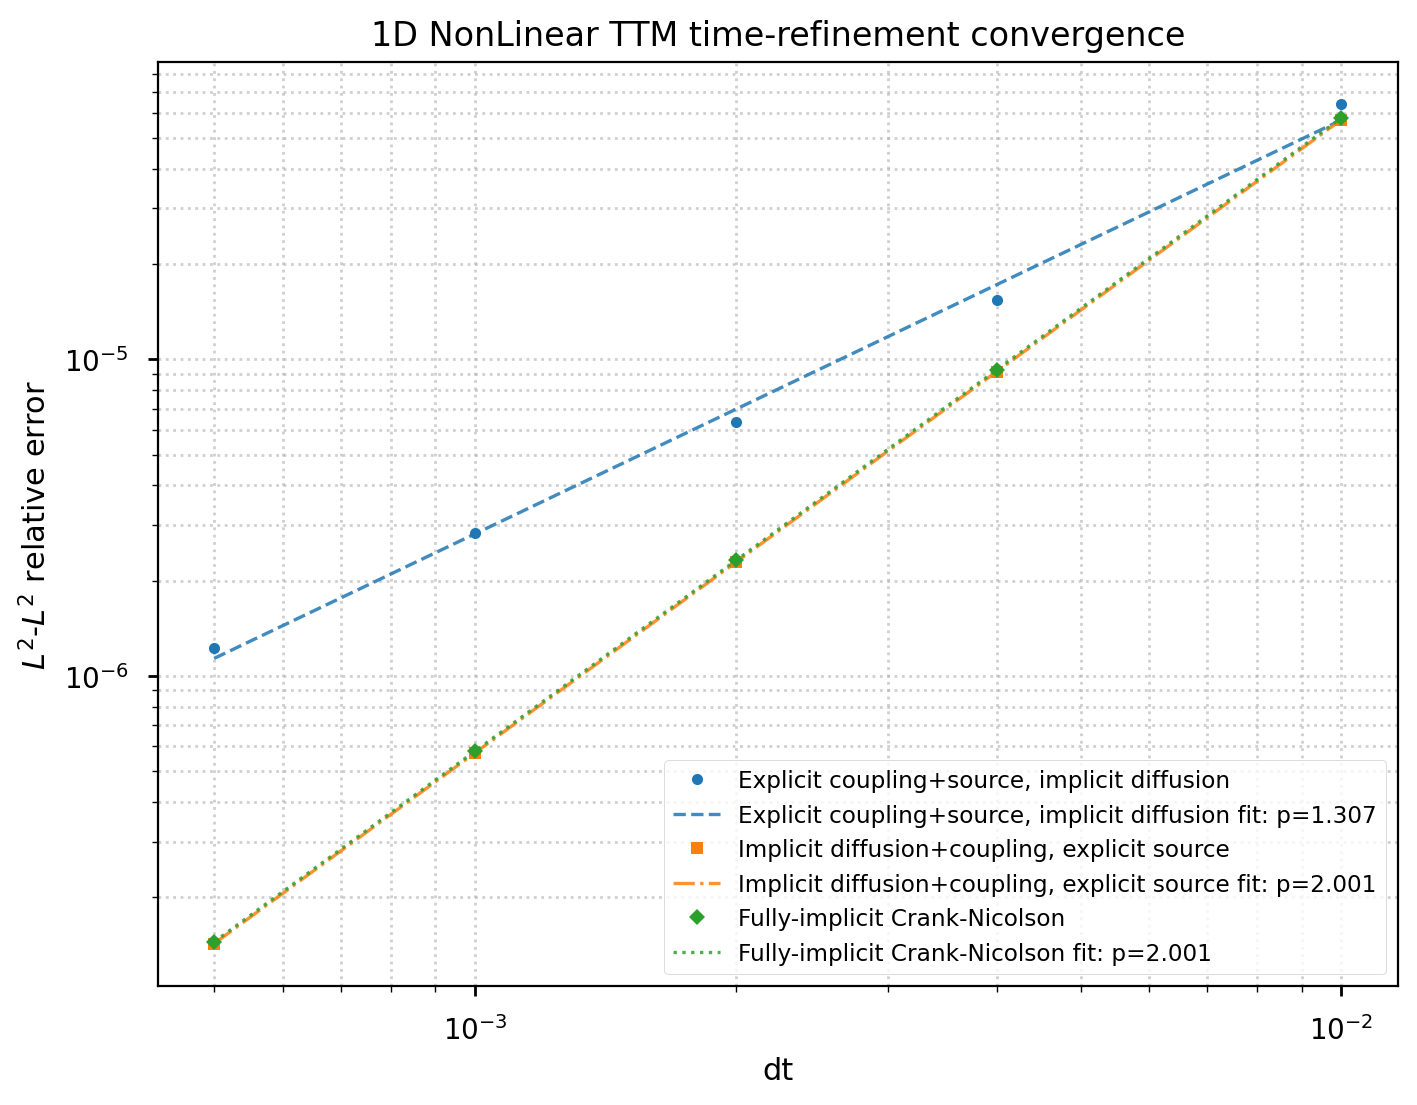
\includegraphics[width=0.48\textwidth]{figures/ch2/time_convergence.png}
    }
    \hfill
    \subfloat[Spatial convergence.\label{fig:ch2-space-convergence}]{
        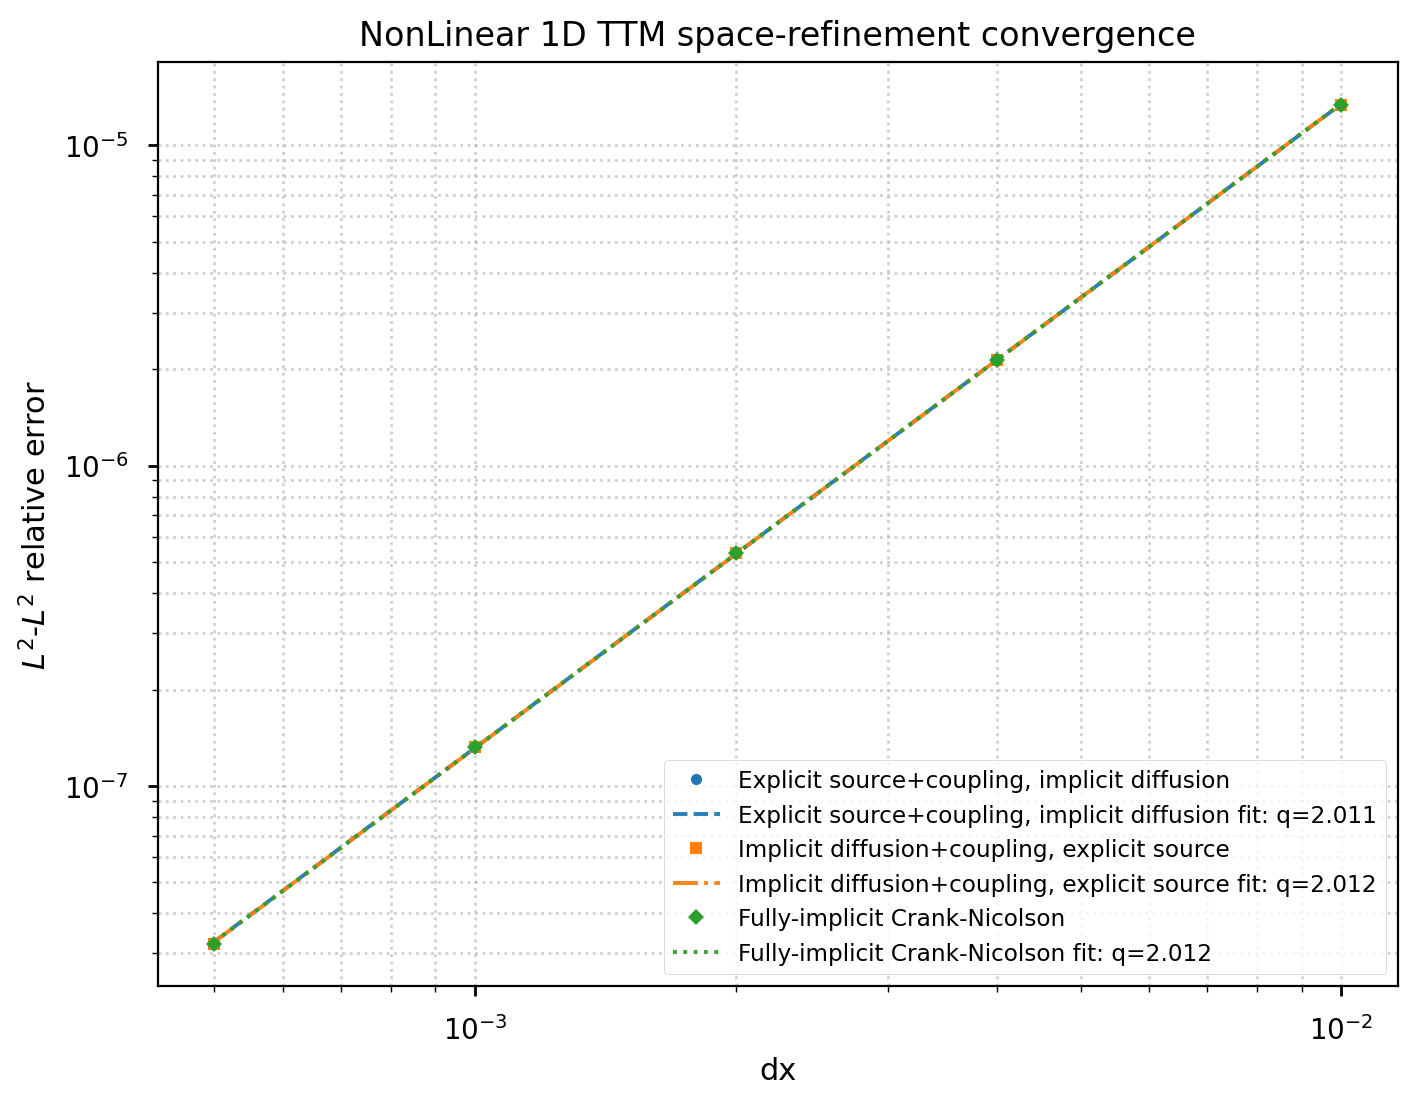
\includegraphics[width=0.48\textwidth]{figures/ch2/space_convergence.png}
    }
    \caption{Convergence study for three IMEX splits of the 1D nonlinear pTTM. Log-log plots of the normalised \(\ell^2\)--\(L^2\) error against \(\Delta_t\) (left) and \(\Delta_x\) (right). The IMEX variant with implicit diffusion and coupling, explicit source (variant 2) achieves the observed second-order behaviour \(p \approx 2\) in both time and space.}
    \label{fig:ch2-convergence}
\end{figure}

The runtime comparison between the three IMEX splits is reported in Table~\ref{tab:ch2-wallclock}. Each row corresponds to five independent runs of the one-dimensional nonlinear solver under the benchmark setup used for the convergence study.
\begin{table}[htbp]
    \centering
    \caption{Wall-clock runtimes for repeated runs of the three IMEX splits.}
    \label{tab:ch2-wallclock}
    \begin{tabular}{@{}lrrrrrr@{}}
        \toprule
        IMEX variant                                   & I     & II    & III   & IV    & V     & Mean           \\
        \midrule
        Explicit coupling + source, implicit diffusion & 32.63 & 32.74 & 32.12 & 32.93 & 32.02 & \textbf{32.49} \\
        Implicit diffusion + coupling, explicit source & 23.67 & 22.89 & 24.33 & 24.25 & 23.42 & \textbf{23.71} \\
        Fully-implicit Crank--Nicolson                 & 27.98 & 28.33 & 26.56 & 26.67 & 26.80 & \textbf{27.27} \\
        \bottomrule
    \end{tabular}
\end{table}

Tables~\ref{tab:ch2-time-convergence} and \ref{tab:ch2-space-convergence} show that the IMEX variant with implicit diffusion and coupling, explicit source attains the observed second order in both variables: the fitted temporal order is \(p \approx 2.001\), identical to the fully implicit Crank--Nicolson reference, and the fitted spatial order is \(p \approx 2.012\) for both schemes. The runtime advantage is nevertheless measurable. Table~\ref{tab:ch2-wallclock} shows that variant~2 is approximately \(1.15\times\) as fast as fully implicit Crank--Nicolson (\(23.71\) s versus \(27.27\) s), because the source Jacobian does not need to be assembled or solved implicitly. By contrast, the explicit-coupling variant suffers a marked deterioration in temporal behaviour, with fitted order only \(p \approx 1.31\) in Table~\ref{tab:ch2-time-convergence}. In that split, the explicit part contains the electron--lattice coupling contribution \(c_1\Delta_t = \mathcal{O}(1)\), so the explicit update is exposed to the stiff exchange scale that the preferred split treats implicitly. The same variant also requires more nonlinear work in practice, with roughly \(3\)–\(4\) Picard iterations per timestep instead of the \(1\)–\(2\) iterations observed for the preferred split. The IMEX variant with implicit diffusion and coupling, explicit source is therefore the scheme of choice throughout this thesis: it exhibits second-order behaviour in the refinement study, keeps the stiff diffusion and coupling terms implicit, and remains computationally efficient.
